\section{Evidence Across Development and Held-Out Cohorts}
\label{sec:v14-evidence}
\subsection{Development evidence and stronger same-data models}
% evidence: configs/final_robustness_v9.json; paper/generated/evidence_argument_v10/decomposition_maximum_dose.csv; paper/generated/evidence_v14/all_results.csv
The protocol was developed on EmoEEG-MC (30 participants, 42 stimuli;
valence/arousal) and Urban Appraisal (62 participants, 56 images; valence)
\citep{openneuro_ds005540,openneuro_ds006850}. The original complete resource
grids cover band-power Ridge, frozen LaBraM and EEGNet under two bounded
settings each. All 12 development-grid intervals include zero under the
five-block fixed-fit analysis. These cohorts were already inspected, and
Urban appraisal is not an identical emotion-induction replication. Their full
grids, interval calibration and historical sensitivity checks remain in
Appendix~\ref{app:development-v13}.

% evidence: paper/generated/evidence_v14/all_results.csv
To address the frozen-encoder limitation, existing v14 runs adapted LaBraM's
last four transformer blocks, final normalization and regression head with
five seeds. The mean matched increments are $-0.0413$ in EmoEEG-MC and
$-0.0418$ in Urban (Table~\ref{tab:v14-primary}). These are negative
same-data sensitivities with one fixed identity partition; they do not inherit
FACED's prospective equivalence interpretation or become independent cohorts.

\subsection{FACED: a locked design on a previously unused cohort}
% evidence: docs/confirmatory_faced_v14_protocol.md; docs/confirmatory_faced_structural_amendment_v14.md; docs/faced_ingestion_summary_v14.json; docs/faced_assignment_summary_v14.json
Before accessing FACED EEG samples or trial ratings, we locked source
eligibility, resource doses, models, exclusions, estimands and equivalence
margins. We used pinned NEMAR FACED v1.1.3 \citep{chen2023faced,nemar2026faced}:
123 participants, 28 videos and 3,444 eligible trials, with no post-outcome
exclusions. A header-only amendment harmonized two channel schemas to 30
scalp channels. Each trial uses the last 30 seconds ending at video offset,
common-average reference, a 0.5--45 Hz bandpass and 100 Hz resampling. Valence
and arousal self-ratings are mapped from $[0,7]$ to $[-1,1]$.

% evidence: configs/confirmatory_faced_v14_experiment.yaml; docs/confirmatory_faced_v14_protocol.md; scripts/run_eegnet_v14.py; scripts/run_labram_peft_v14.py
Five participant folds crossed with four stimulus folds cover every eligible
trial once per rotation. Five independently hashed rotations require full
refitting, producing 100 splits; every split uses the complete
$\{0,1,2,4,8\}^2$ resource grid. EEGNet uses validation-selected learning rate
and training duration. LaBraM adapts its final four blocks, normalization and
head. Both use the same five frozen training seeds and post-fit calibration
rule. Test labels select neither checkpoints nor hyperparameters. Positive
resource doses deliberately expose the corresponding identity, so these cells
are resource-conditioned deployments rather than zero-shot identity tests.

% evidence: paper/generated/evidence_v14/all_results.csv; src/openaffect_eeg/training_uncertainty.py
The FACED primary statistic averages matched CCC differences over all resource
cells and both targets. Joint intervals reuse the already executed predictions
and share participant--stimulus multiplicities while resampling training seeds
and complete refit rotations. This includes the executed training procedures,
not uncertainty over arbitrary architectures or tuning policies. All observed
analyses have 2,000 valid draws. The pre-outcome primary margin is
$\pm0.05$ CCC, with $\pm0.025$ as a stricter sensitivity; equivalence requires
the 90\% decision interval to lie inside the margin. These are benchmark
resolution choices, not clinically validated thresholds. A grid-average
equivalence statement does not certify each target, participant or cell.

% evidence: paper/generated/evidence_v14/all_results.csv
\begin{table}[t]\centering\small
\caption{Existing five-seed adapted-model evidence. FACED intervals jointly resample participants, stimuli, executed training seeds and five fully refitted rotations; development-task intervals hold their single rotation fixed. Equivalence decisions apply to the uniform-grid mean and use the 90\% interval. Failed locked controls limit the FACED confirmation claim.}
\label{tab:v14-primary}
\setlength{\tabcolsep}{3pt}
\begin{tabularx}{\linewidth}{@{}l l r X l@{}}\toprule
Dataset & Model & $\Delta$CCC & 95\% interval & Decision\\\midrule
FACED & EEGNet & $-0.0414$ & $[-0.0875, +0.0002]$ & uncertain \\
FACED & LaBraM tail & $-0.0053$ & $[-0.0112, +0.0009]$ & equivalent$^{*}$ \\
EmoEEG-MC & LaBraM tail & $-0.0413$ & $[-0.0690, -0.0112]$ & negative \\
Urban & LaBraM tail & $-0.0418$ & $[-0.0755, -0.0064]$ & negative \\
\bottomrule\end{tabularx}
\vspace{2pt}\parbox{\linewidth}{\footnotesize $^{*}$FACED LaBraM also meets the narrower $\pm0.025$ margin. Development-task margins were not prespecified and are not used for a confirmatory equivalence claim.}
\end{table}


% evidence: paper/generated/evidence_v14/all_results.csv
Adapted LaBraM's FACED mean is $\FacedLabramMean$ (95\% interval
$\FacedLabramCI$; 90\% interval $\FacedLabramDecisionCI$), within both
equivalence bounds. EEGNet's mean is $\FacedEegnetMean$ (95\% interval
$\FacedEegnetCI$); its 90\% interval $\FacedEegnetDecisionCI$ crosses the
lower equivalence bound, leaving the decision inconclusive. The two models
therefore support different levels of precision, not a universal absence of
EEG information. These statistical decisions remain conditional on the
declared design; the failed controls below limit a fully confirmatory reading.

% evidence: paper/generated/evidence_v14/archive/faced_eegnet_observed/cells.csv; paper/generated/evidence_v14/archive/faced_labram_observed/cells.csv; paper/generated/evidence_v14/resource_corners.csv
\begin{figure}[t]\centering
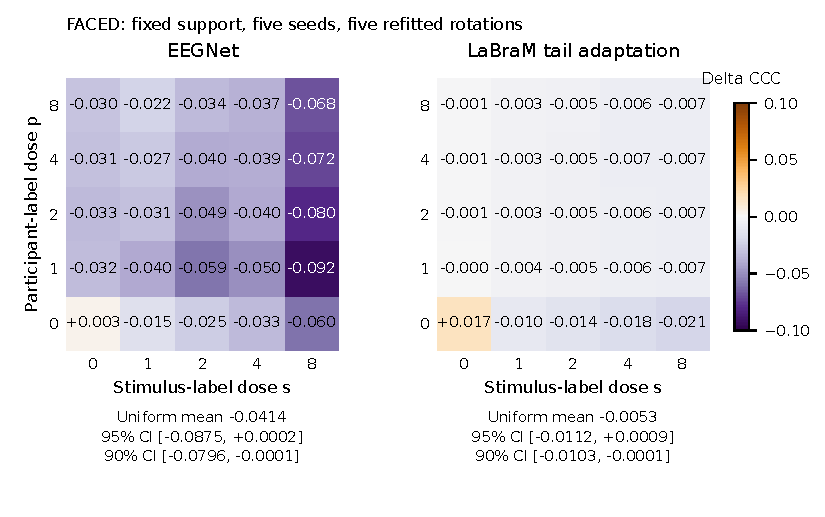
\includegraphics[width=\linewidth]{../generated/evidence_v14/faced_matched_heatmap.pdf}
\caption{The complete FACED matched-increment grids. Positive values favor EEG;
the shared scale and printed values retain dose heterogeneity. Displayed zeros
are rounded, not exact equality. Each cell
averages paired differences over executed seeds, rotations and targets on
identical test support. Intervals below each grid describe the uniform mean.
Pointwise and simultaneous cell bands are released separately; the heatmap
does not establish cellwise equivalence. Negative and failed positive controls
are reported in Table~\ref{tab:v14-controls}.}
\label{fig:faced-v14}
\end{figure}

% evidence: paper/generated/evidence_v14/resource_corners.csv
The heatmap exposes a boundary hidden by the mean. At zero participant
calibration, LaBraM's point increment changes from $+0.0170$ with no
same-stimulus labels to $-0.0212$ with eight such labels. At the corresponding
zero-stimulus corners, its increment is $+0.0170$ at participant dose zero and
$-0.0008$ at dose eight. All four corners for both architectures are released,
without choosing cells by sign. These are descriptive changes under different
contracts, not a tested causal effect of label acquisition or proof that a
particular cell has no EEG signal.

\subsection{Negative controls, failures and post-failure recovery}
% evidence: paper/generated/evidence_v14/all_results.csv; docs/confirmatory_positive_control_amendment_v14.md
Full-grid label permutations give mean increments $-0.0400$ (EEGNet) and
$-0.0058$ (LaBraM). Neither triggers the prespecified spurious-positive
warning; the similarity to observed estimates is descriptive, not a formal
observed-versus-permuted test. Two completed EEGNet sinusoidal positive
controls failed: raw-target encoding gave $-0.1476$, and residual-aligned
encoding gave $-0.0562$, below the required $+0.10$ gate. Thus target alignment
alone did not explain the failure. Both failures and their intervals remain
in Table~\ref{tab:v14-controls}.

% evidence: paper/generated/evidence_v14/all_results.csv; docs/confirmatory_positive_control_amendment_v14.md
After observing those failures, signed-power controls separated positive and
negative residual magnitudes across channels to avoid crop-dependent carrier
phase ambiguity. A frozen, cost-controlled subset recovered $+0.6512$ with
EEGNet and $+0.6303$ with LaBraM. It covers five selected splits, three stimulus
doses and all participant doses and training seeds, not the full crossed test
support. The earlier 52-fit incomplete full-grid attempt is retained and
excluded from inference. These results show sensitivity to a redesigned,
strong injected signal; they neither establish optimal use of real EEG nor
retroactively repair the failed locked controls. FACED is an unused cohort
with a prospectively locked observed-data design, but the complete pipeline
does not meet a fully preregistered confirmation claim.

\section{What the Evaluation Changes in Practice}
\label{sec:practical-cases}
% evidence: paper/generated/evidence_v14/system_attribution_cases.csv
\begin{table}[t]\centering\small
\caption{Existing maximum-dose LaBraM R1 cases: point CCC contrasts. Changing the comparator changes the attribution. None of the total or matched endpoint ranges establishes a positive gain; full conditional ranges and other settings are retained in the development appendix.}
\label{tab:v14-cases}
\begin{tabularx}{\linewidth}{@{}lXXX@{}}\toprule
Task & System $EC-P$ & Calibration $PC-P$ & Matched EEG $EC-PC$\\\midrule
EmoEEG-MC & $+0.0961$ & $+0.1420$ & $-0.0459$ \\
Urban & $+0.0587$ & $+0.0774$ & $-0.0186$ \\
\bottomrule\end{tabularx}
\end{table}

% evidence: paper/generated/evidence_argument_v10/decomposition_maximum_dose.csv
\paragraph{Case 1: attributing an apparent system gain.}
At the predeclared maximum resource dose, the frozen LaBraM R1 system improves
on the uncalibrated prior by $+0.0961$ CCC in EmoEEG-MC and $+0.0587$ in
Urban. Supplying exactly the same calibration labels to the EEG-free
comparator yields $+0.1420$ and $+0.0774$, leaving matched EEG differences
$-0.0459$ and $-0.0186$. The original positive point estimate describes the
system package; it does not identify added EEG value. Even the total-gain
intervals include zero, so this is not a reversal of an established
significant benefit. Appendix~\ref{app:development-v13} reports all settings
and the descriptive endpoint ranges. The practical correction is to change
the comparator and attribution, not to claim that a deployed sensor is
unnecessary.

% evidence: paper/generated/evidence_v14/resource_corners.csv; paper/generated/evidence_v14/all_results.csv
\paragraph{Case 2: distinguishing calibration regimes.}
A single zero-resource comparison cannot answer what EEG adds after repeated
stimulus labels become available. FACED's LaBraM surface ranges from positive
to negative point increments across those shared budgets, while its complete
uniform mean meets the fixed equivalence margins. Reporting the grid makes
the budget assumption visible and prevents promoting the mean to an
equivalence certificate for a selected deployment cell. This is the empirical
consequence of adding a stimulus axis to a participant-only baseline.

% evidence: paper/generated/submission_closure_v11/external_claim_repair.json; paper/generated/final_closure_v9/external_audit/public_summary.json
\paragraph{Case 3: narrowing an external execution claim.}
For the same pinned EEGain split function and eligible trial universe, the
checker blocks all five requests that jointly require held-out test
participants and training--validation trial isolation. The same five traces
allow the narrower held-out-test-participant claim. Generated marker windows
carry lineage only; no external emotion classifier was retrained. This
source-linked case changes a checkable claim about executed partitions, not
the validity of EEGain's published model scores. Separate synthetic faults
test resource parity and missing provenance; they are not attributed to
external authors. The reusable interface accepts trial identities, executed
resource records and explicit requirements, and returns \texttt{allow},
\texttt{block} or \texttt{unverifiable} with failed checks.
